
\documentclass{beamer}
\usetheme{Madrid}
\usepackage[utf8]{inputenc}
\usepackage[spanish]{babel}
\usepackage{amsmath}
\usepackage{graphicx}
\usepackage{lmodern}

\title{Análisis Predictivo y Gestión de Datos}
\subtitle{Sesión 5: Regresión Logística}
\author{Oscar Leonardo Rincón León}
\date{\today}

\begin{document}

\frame{\titlepage}

\begin{frame}{Objetivo de la sesión}
\begin{itemize}
    \item Entender la lógica de la regresión logística y su función sigmoide.
    \item Usarla para clasificar de forma binaria: conectividad baja vs. alta.
    \item Evaluar su rendimiento con métricas como precisión, F1-score y curva ROC.
\end{itemize}
\end{frame}

\begin{frame}{¿Por qué no usar regresión lineal para clasificación?}
\begin{itemize}
    \item La regresión lineal predice valores continuos sin límite.
    \item Para clasificación necesitamos probabilidades entre 0 y 1.
    \item La regresión logística lo soluciona usando la función sigmoide.
\end{itemize}
\end{frame}

\begin{frame}{¿Qué es la regresión logística? (1/2)}
\begin{itemize}
    \item Modelo de clasificación binaria.
    \item Predice la probabilidad de que una observación pertenezca a la clase 1.
    \item Usa una combinación lineal de las variables:
    \[
    z = \beta_0 + \beta_1 x_1 + \dots + \beta_n x_n
    \]
\end{itemize}
\end{frame}

\begin{frame}{¿Qué es la regresión logística? (2/2)}
\begin{itemize}
    \item Aplica la función sigmoide a $z$:
    \[
    \text{P}(y=1 \mid x) = \frac{1}{1 + e^{-z}}
    \]
    \item La salida es una probabilidad entre 0 y 1.
    \item Se predice clase 1 si $P \geq 0.5$ (o se ajusta el umbral).
\end{itemize}
\end{frame}

\begin{frame}{Visualización de la función sigmoide}
\begin{itemize}
    \item Transforma cualquier valor real a una probabilidad.
    \item Representa la probabilidad de clase positiva.
\end{itemize}
\begin{center}
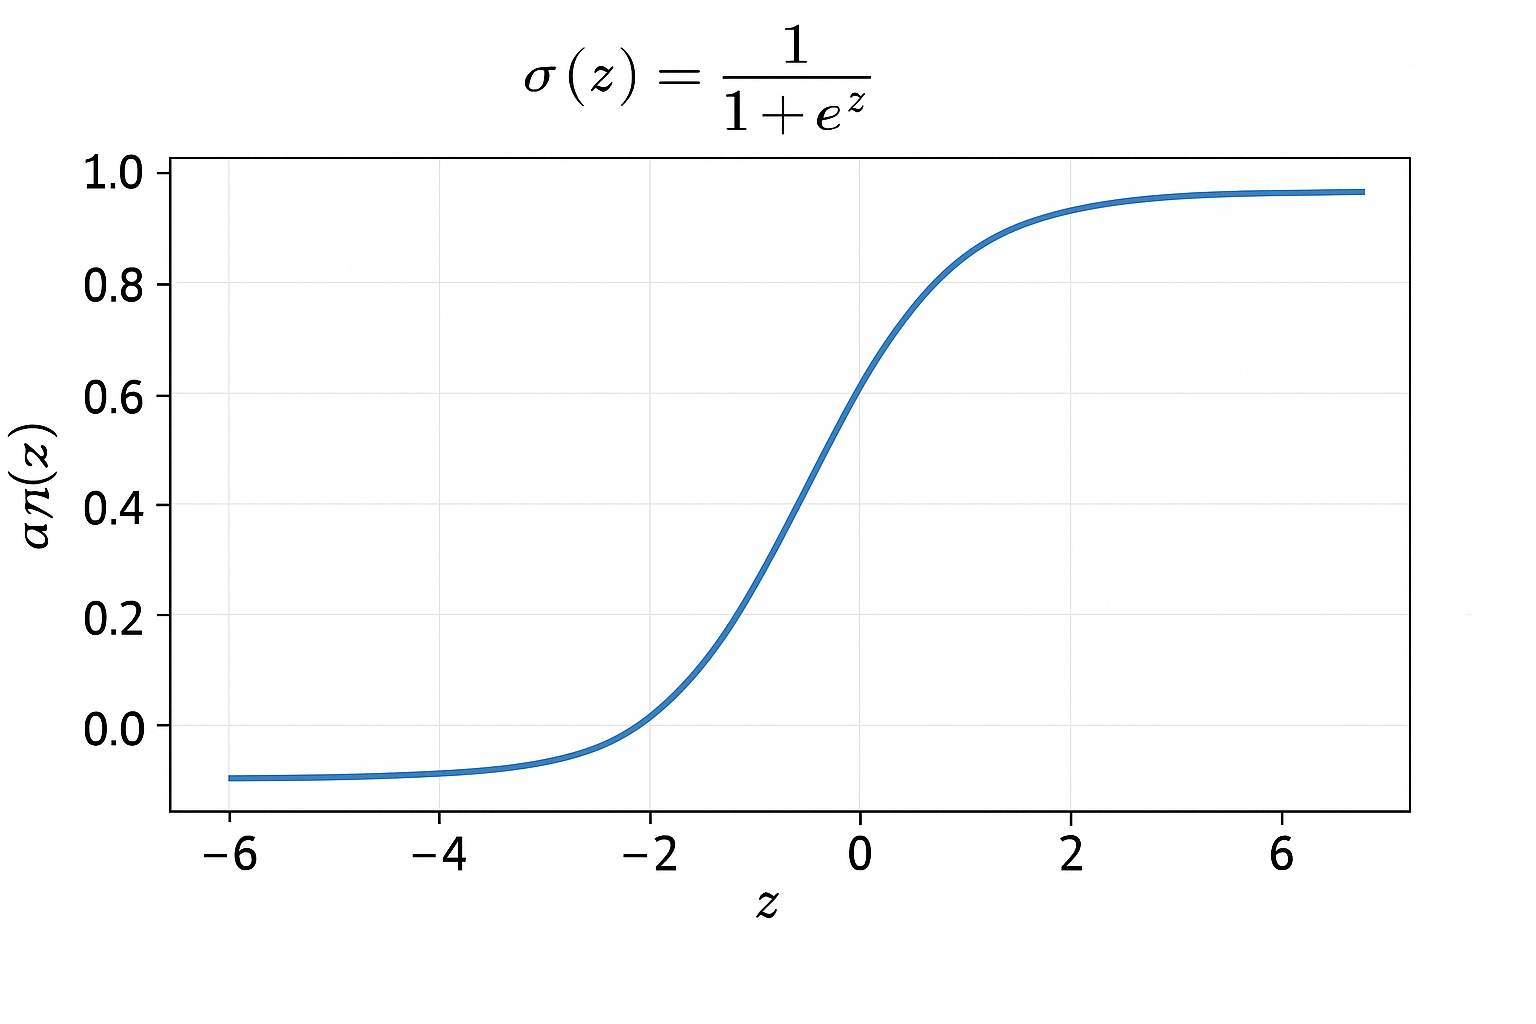
\includegraphics[width=0.5\textwidth]{sigmoid_example.png}
\end{center}
\end{frame}

\begin{frame}{¿Qué son los odds y el logit?}
\begin{itemize}
    \item \textbf{Odds:} cociente entre la probabilidad de éxito y de fracaso:
    \[
    \text{odds} = \frac{p}{1 - p}
    \]
    \item \textbf{Logit:} logaritmo de los odds:
    \[
    \log\left(\frac{p}{1 - p}\right) = z
    \]
\end{itemize}
\end{frame}

\begin{frame}{Interpretación de los coeficientes}
\begin{itemize}
    \item Un aumento de 1 unidad en $x_i$ incrementa los \textbf{log-odds} en $\beta_i$.
    \item En términos de odds:
    \[
    \text{odds nuevos} = \text{odds actuales} \times e^{\beta_i}
    \]
    \item La relación con la probabilidad no es lineal (curva sigmoide).
\end{itemize}
\end{frame}

\begin{frame}{Evaluación del modelo}
\begin{itemize}
    \item Métricas comunes:
    \begin{itemize}
        \item Precisión, Recall, F1-score
        \item Matriz de confusión
        \item Curva ROC y AUC
    \end{itemize}
    \item Se puede ajustar el umbral para mejorar el rendimiento en clase minoritaria.
\end{itemize}
\end{frame}

\begin{frame}{Ventajas de la regresión logística}
\begin{itemize}
    \item Fácil de entrenar e interpretar.
    \item Permite estimar probabilidades.
    \item Buen punto de partida antes de usar modelos más complejos.
\end{itemize}
\end{frame}

\begin{frame}{Cierre}
\begin{itemize}
    \item La regresión logística modela probabilidades para clasificación binaria.
    \item Puede expresarse como función sigmoide o como logit.
    \item Es evaluada con precisión, F1 y curvas ROC.
\end{itemize}
\end{frame}

\end{document}
